\label{fs-acker-preliminaries}

\subsection{Overview}

\tracker\ framework bases on another idea of the propagation the fact that the substream ends. Instead of injecting special elements directly into the dataflow, we design a special agent (process) that:

\begin{enumerate}
    \item Receives signals that a substream terminated from data producers.
    \item Watches for in-flight elements and if they belong to some substream.
    \item Notifies dataflow processes when the substream ends {\em for them}, i.e., when they do not receive any elements which satisfy some predicate.
\end{enumerate}

\begin{figure}[htbp]
  \centering
  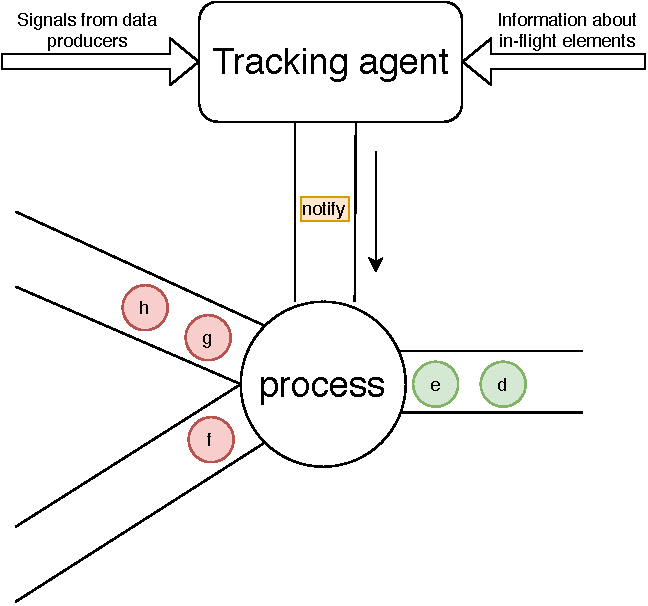
\includegraphics[width=0.50\textwidth]{pics/tracker-scheme.pdf}
  \caption{\tracker\ framework: an example}
  \label{tracker_scheme}
\end{figure}

The general scheme of the \tracker\ mechanism is shown in Figure~\ref{tracker_scheme}. Special (possibly distributed) {\em tracking agent} receives signals from data sources, fetches information about in-flight elements, and then decides to send notifications about substream end. Before diving into implementation details, we should answer the following questions regarding \tracker\ framework, as explained in the next subsection.

{\bf Q1 How to organize monitoring of in-flight elements?} To notify processes that a substream ends, the tracking agent should receive the corresponding signal from data producers and ensure no in-flight elements belong to the substream. 

{\bf Q2 How to reveal the exact moment when the substream ends?} Unlike punctuations, \tracker\ notifications are completely async with dataflow elements because they go through another network channel. Hence, dataflow items and notifications are not ordered, making it hard to determine an exact event that finishes a substream.

{\bf Q3 What are the functional and performance properties of \tracker?} \tracker\ framework is designed to eliminate the restrictions of punctuations framework. We should demonstrate that it is suitable for cyclic dataflows as well as can provide lower network overhead.

\subsection{Discussion}

\subsubsection{Answering Q1: How to organize monitoring of in-flight elements?}
Assume that each process sends to tracking agent the following information about each sending or receiving event $e = <action,m>$:
\begin{enumerate}
    \item $action$: send or receive.
    \item $pred(m)$: the result of applying a substream predicate.
    \item process identifier.
\end{enumerate}

Note that the result of applying predicates can be a vector if we are tracking multiple substreams. Process identifier is an optional field that can be used to send notifications independently for various processes or parts of the physical graph. We will discuss it in detail in the next section.

Using this information along with signals from data producers, the tracking agent can detect when there is a guarantee that a substream ends and send a corresponding notification $e^{n} = <send,pred(m)>$. Therefore, function $S(E_{proc})$ for \tracker\ framework is the following:

\begin{align*}
& S_{tracker}(E_{proc}) = \exists e \in E_{proc} : e = \langle recv,pred(m)\rangle_{tracker,p}
\end{align*}

Note that the correctness of the general guarantee for \tracker\ depends on the implementation of the tracking agent detailed in the next section. The formal proofs that function $S_{tracker}(E_{proc})$ along with the \tracker\ implementation satisfy the general guarantee are in the appendix~\ref{appendix:tracker-proof}.

\subsubsection{Answering Q2: How to reveal the exact moment when the substream ends?}

\subsubsection{Answering Q3: What are the functional and performance properties of \tracker?}
% To determine an exact event that finishes a substream, one can define an order between notifications and dataflow items.